\documentclass {article}
\usepackage{fullpage}
\usepackage{graphicx}
\usepackage{hyperref}

\begin{document}

~\vfill
\begin{center}
\Large


\textbf{Pokemon Fight! Pikachu VS Snorlax}

Name: Zhenyan Zhu

Student ID: 20817494

User ID: z277zhu

December 2, 2022
\end{center}
\vfill ~\vfill~
\newpage
\section{General}
The purpose of this project was to implement a extendable 3D Pokemon battle game. I feel that I have
successfully met all of my goals and even add other extra features to make this an complete game. \\
This game requires you to control Pikachu and defeat the Boss - Snorlax. You should circumvent from Snorlax's attack, including
Body Slam and Meteorite fall and attack Snorlax by discharging.


\section{Project Structure}
    /docs : project report and proposal \\
    /lib : static and shared third party libraries  \\
    /shared: source code of third party libraries \\
    /src: source code of project \\
    \indent /src/Assets : shaders, textures, audios, lua modelling, .obj files \\
    \indent /src/include: include files (*.hpp) of project \\
    \indent /src/src: implementation files (*.cpp) of project \\
    \indent /src/modelling: modified A3 source code for collecting animation assets 

\section{Code Mapping}
\begin{enumerate}
    \item Animation system (src/src/Animation.cpp, src/include/Animation.hpp)
    \item Particle systems that can be used by Lua scripts  (src/src/particle.cpp, src/include/particle.hpp, src/src/scene\_lua.cpp)
    \item Texture importing and caching system that can be used Lua scripts (src/src/texture.cpp, src/include/texture.hpp, src/src/scene\_lua.cpp)
    \item Shadow (Assets/shadow\_depth.fs, Assets/shadow\_depth.vs, Assets/Pong.fs, src/src/shadow.cpp, src/include/shadow.hpp, src/src/GameWindow.cpp)
    \item Grass (Assets/grass.fs, Assets/grass.geo, Assets/grass.vs src/src/GameWindow.cpp)
    \item Sound (src/src/GameWindow.cpp, src/src/sound.cpp, src/include/sound.hpp)
    \item Pokemon behaviors (src/src/GameObject.cpp, src/include/GameObject.hpp)
    \item Scene modelling, Pokemon modelling (Assets/Scene.lua, Assets/pikachu.lua, Assets/snorlax.lua)
\end{enumerate}

\section{Manual}
    \subsection{Build}
    On Linux, run 'bash build\_linux.sh' at the root of project; on Mac, run 'bash build\_mac.sh'
    \subsection{Run}
    cd src \&\& ./game
    \subsection{Game Control}
    \begin{enumerate}
        \item  \textbf{Movement:} The movement of Pikachu is controlled by keyboards. Similar to other games, 'W' controls Pikachu to move up; 'A' controls Pikachu to move left;
        'S' controls Pikachu to move down; 'D' controls Pikachu to move right.
        \item \textbf{Attack:} Press 'j' to use discharge from Pikachu's left hand; press 'k' to use discharge from Pikachu's right hand.
        \item \textbf{Others:} Press 'q' to quit the game; press 't' to enable/disable toon shading.
    \end{enumerate}
    \subsection{Output}
    There will be no command-line output when the debug mode is off.
    \newpage
   
    



\newpage

\section{Implementation}
I listed several interesting technical points that I found most challenging and spent a large amount of time designed and implemented. For other parts, please refer to my 
project proposal for technical contents.
\subsection{Animation System}
This section describes the design and implementation of my animation system. (src/src/Animation.cpp;src/include/Animation.hpp) \\
The following UML diagram describes a high-level view of the components of the system (some getter and setter are omitted).\\
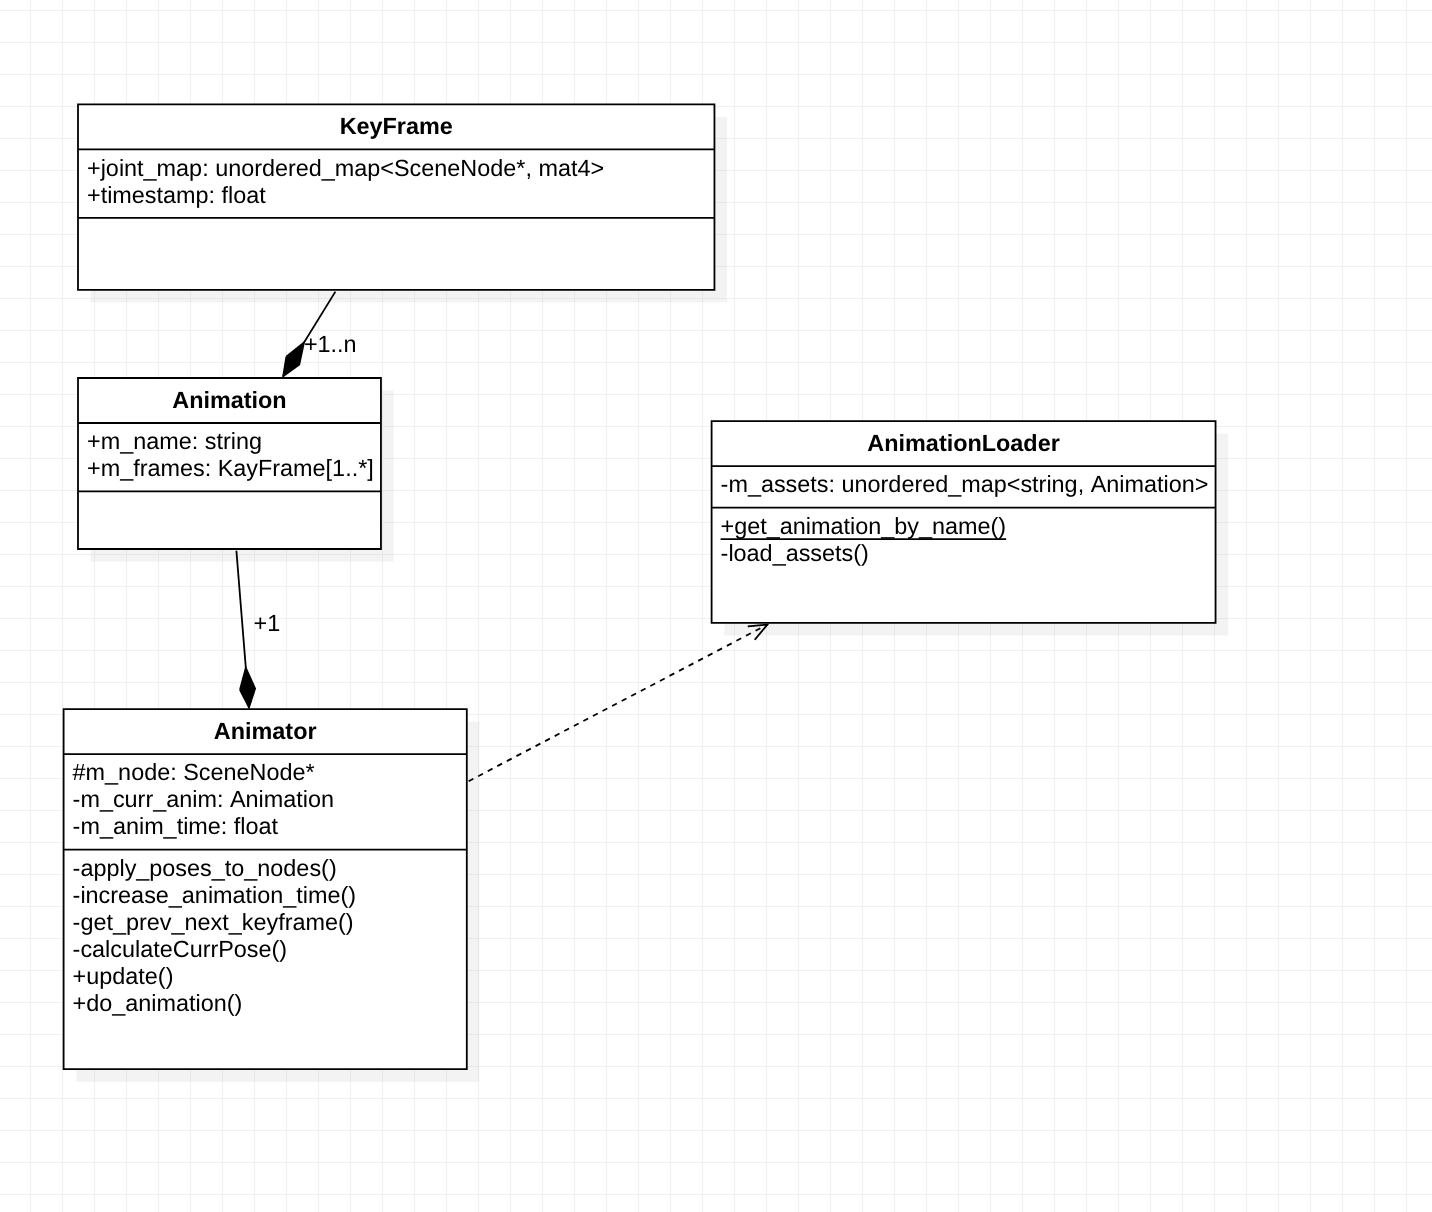
\includegraphics[width=100mm]{uml_animation.png} \\
I would like to mainly introduce the AnimationLoader and the Animator class.
\begin{enumerate}
    \item \textbf{AnimationLoader}: It is a Singleton that holds the assets of all animations. \\
    in the beginning of the game, the AnimationLoader will load animations of Pikachu and Snorlax from Assets/*.ani files. *.ani file has the following protocols: \\
        \${animation1Name}\$ \${num of keyframes}\$  \\
        \indent \${num of nodes in frame 1}\$ \${timestamp at frame 1}\$    \\
        \indent \indent \${name of node 1}\$ \$quat.w\$ \$quat.x\$ \$quat.y\$ \$quat.z\$ \$trans.x\$ \$trans.y\$ \$trans.z\$ \\
        \indent \indent ... \\
        \indent \indent \${name of node n} \\
        \indent ... \\
        \indent \${num of nodes in frame m}\$ \${timestamp at frame k}\$    \\
        \${animation2Name}\$ \${num of keyframes}\$  \\
        ... \\
       All the animations will be loaded into the m\_assets field of the AnimationLoader, which is an unorder\_map such that we can 
       lookup an animation by name with runtime O(1)
    \item \textbf{Animatior}: It is the class that perform the updates of an animation.
    \begin{enumerate}
        \item To perform an animation, \textit{do\_animation(Animation* ani\_ptr)} will be invoked. \textit{ani\_ptr} is a pointer points to an animation that holds by the AnimationLoader. When
        set the animation to \textit{m\_curr\_anim}, despite clean the current animation and copy all the fields from the ani\_ptr, it will also fetch the frame 0, which is the current pose
        of the nodes defined in frame1 into the current animation for the interpolation calculation in \textit{update()}. It will also set the current time of the animation.
        \item the \textit{update()} method will be called in each frame that calculates the current pose and apply to the all related SceneNodes. It has the following procedures:
        \begin{enumerate}
            \item It will update the current timestamp after do\_animation() is called time by utilizing the routines in timestamp.hpp.
            \item It will fetch the current and next keyframes by calling \textit{get\_prev\_next\_keyframe}, which takes O(1) because the current frame index is maintained.
            \item It will calculate the current poses, which are the transform matrices of each SceneNode that the current keyframe tracks. \\
                We will first calculate the current progression of the current frame, which is calculated by the formula $progression = \frac{(currentTime-prevKey.timestamp)}{(nextKey.timestamp-prevKey.timestamp)}$ \\
                Then, we calculate the interpolated transformation matrix for each SceneNode at the current progress by calling \textit{glm::interpolate(prevKey.transforms[node], nextKey.transforms[node], progression)} \\
                Finally, we apply the current poses to these SceneNodes by multiplying the difference between the calculated transformation and the current transformation (\textit{calculatedTrans * inverse(currTrans)}) to their current transformations.
        \end{enumerate}
    \end{enumerate}
\end{enumerate}
All the fields and methods of Animator are private, and other components can only invoke the update() or do\_animation() methods, so it's quite encapsulated.

\subsection{Game Objects}
This section will introduce the design and implementation of the core component of the game - the game objects including Pikachu and Snorlax. The following UML gives a high-level
description of the game objects. (src/GameObject.cpp, include/GameObject.hpp, src/AttackUnit.cpp, include/AttackUnit.hpp)\\
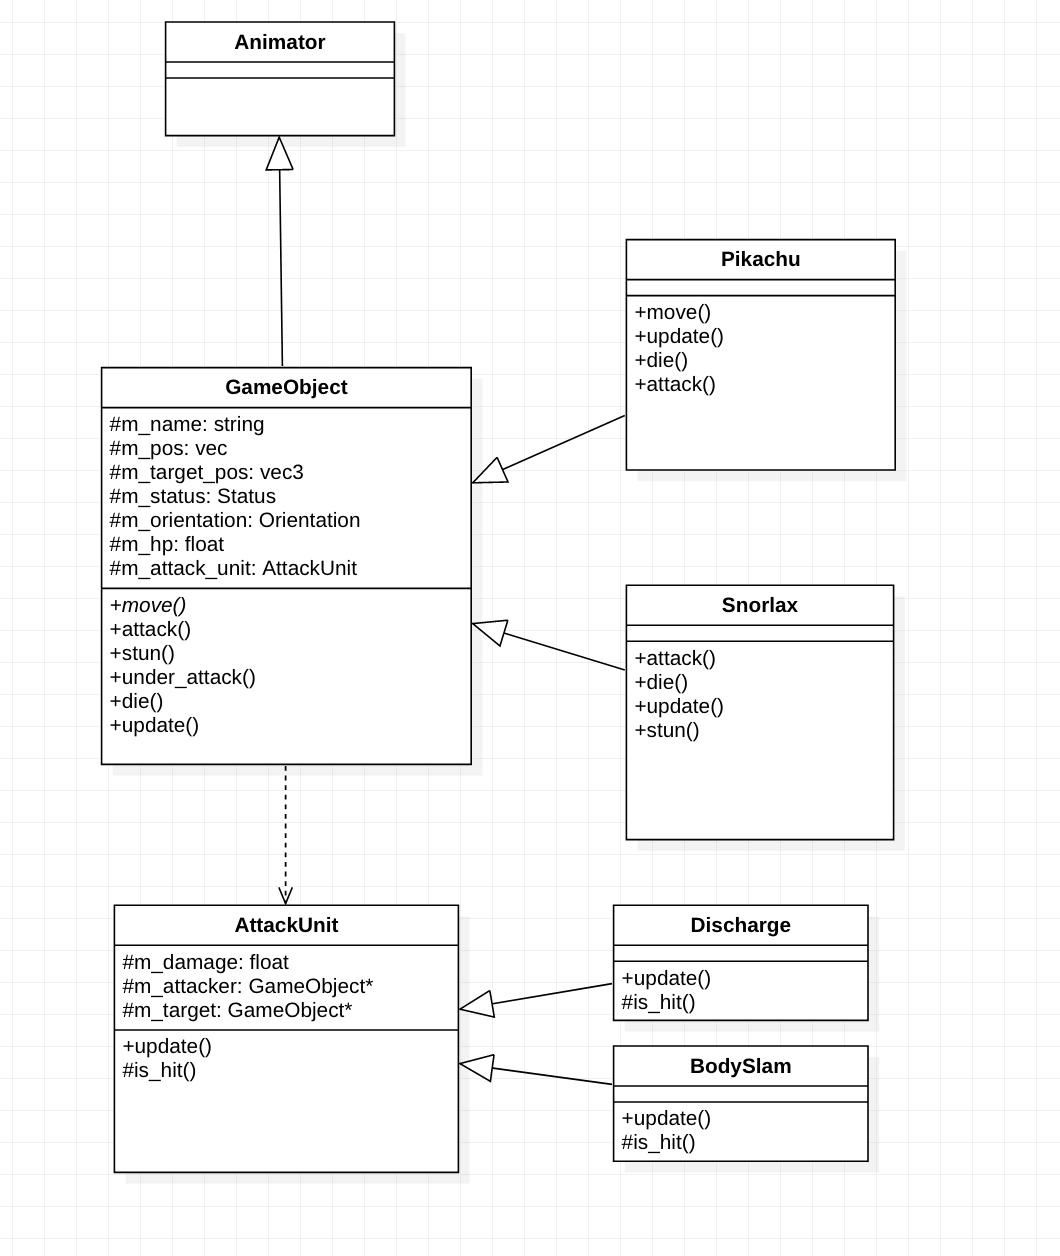
\includegraphics[width=100mm]{uml_gameobject.png} \\
The abstract class \textit{GameObject} is inherit from the Animator class as we talked above because the GameObject is an Animator that we want to interact with. It is highly abstracted as there are only 
5 main methods exposed to other components:
\begin{enumerate}
    \item \textit{move(x,z)}: this method will not directly move the game object with current position + (x, 0, z), but it will only set the \textit{m\_target\_pos} field to be the target position 
    and delegate the work in the \textit{update} method. Pikachu's move will do the corresponding animation; Snorlax cannot move because his BodySlam will help him to move
    \item \textit{attack(name, target)}: this method will instantiate an AttackUnit object and attach it to the \textit{m\_attack\_unit} field and 
    delegate the work of the real attacking in the \textit{update()} method of this attack unit.
    \item \textit{stun()}: this method will be overwritten by Snorlax, after he did BodySlam, stun() will be invoked and he will do the stun animation.
    \\ Pikachu does not have stun()
    \item \textit{under\_attack(damage)}: this method will set the hp of the game object to be $max(0, m_hp-damage)$, when it's lower than 0, it will invoke the die() method and notify the game window to stop the game.
    \item \textit{die()}: this method will set the status of game object to be Status::Dead such and perform the corresponding side effects. For Pikachu, it will be smashed into a pancake. This can be done by scale Pikachu's 
    SceneNode with a scaling factor of (1,0.01, 1); For Snorlax, a die animation will be played.
    \item \textit{update()}: this method overwrites Animator::update(). It will invoke Animator::update() when \textit{m\_status} is not idle(which means the object is performing some tasks with animations).
    \\ Meanwhile, it will also invoke the update() method of m\_attack\_u to update the attack unit. Additionally, it will interpolate the position of the game object when its target position is set.
    \item \textit{AttackUnit::update()}: this method defines the main logic of how a GameObject attack another. Concrete AttackUnit has their own implementation of update.
    \begin{enumerate}
        \item \textit{BodySlam::update()}: When BodySlam is instantiated, it will set the attacker's target position's y component to SKY(100.0f) such that the \textit{GameObject::update()} will eventually move the object to the sky. the update() method has two phases and it will query the position of the attacker in each frame.
        In phase1, if the attack unit found that the game object has touched the sky(pos.y == 100), then it will perform phase2() by setting the x and z components of the attacker's position to the target object's position, and set the attacker's
        target position's y component to the GROUND(y=-8). When it found that the game object touched the ground, it will emit the particle effect of flying dirt, shake the camera and invoke the \textit{under\_attack()} method
        of the target object if hit.

        \item \textit{Discharge::update()}: The discharge will hold a remaining time for instantiating another discharge effect. In each update(), the remaining time will be updated and when it's less than 0,
        it will invoke \textit{lightning\_effect()} to discharge lightning. This forms the effect of the a realistic discharge because. In each frame, the attack unit will also determine whether the ray(lightning) hits the target object or not
        by determine the intersection of a ray to a sphere as we implemented in A4 and generate damage to the target object.
        
    \end{enumerate}
\end{enumerate}

\subsection{Particle Systems \& different particle effects}
This section describes the structure of particle systems and how I implemented different particle effects including flying dirt, lightning and meteorite fall.
(/src/particle.cpp, /include/particle.hpp)
\begin{enumerate}
    \item The ParticleSystem holds a pool of Particles and a index points to the next available particle encapsulated. The other component should invoke the \textit{Emit} method to emit a new particle. \\
    Each Particle has their own position, velocity, rotation, rotation velocity, size, gravity and lifetime with some random noise factors. In ParticleSystem::update(), all the active particles will update their position by their velocity and update
    their velocity by the gravity to achieve the realism.
    \item \textit{dirt\_flying\_effect(radius, position, base\_num)}: After invoking this routine, you would see random numbers of dirts,ranging from base\_num to 1.5 * base\_num,spilled out from the ground at the given position forming a circle with the given radius, then falls onto the ground after a while. Effect is shown below. \\
    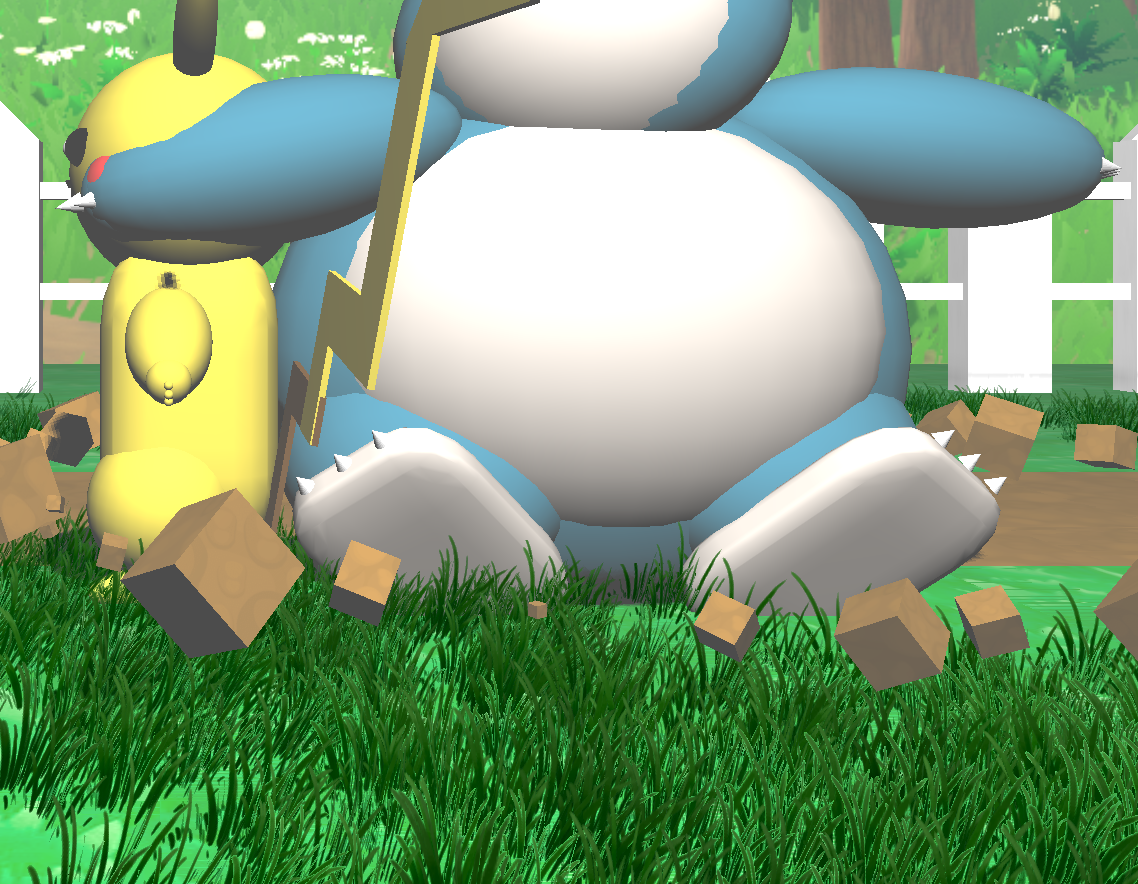
\includegraphics[width=100mm]{flyingdirt.png} \\
    To implement this effect, we first calculate the angle $k$ difference between two dirt square $k = \frac{2\pi}{number of squares}$. Then, for $square_i$, the angle is $\phi = i * k$, the x position is position.x + radius * $cos(\phi)$, the z position is position.z + radius * $sin(\phi)$, the velocity will be
    normalize($square_i$ - position) + vec3(0,10,0) to make the squares have an effect of spilling out from the given position. 
    \item \textit{lightning\_effect(position, dir)}: After invoking this routine, you should see a lightning beam emitted from a given position with some randomly generated electrons nearby. \\
    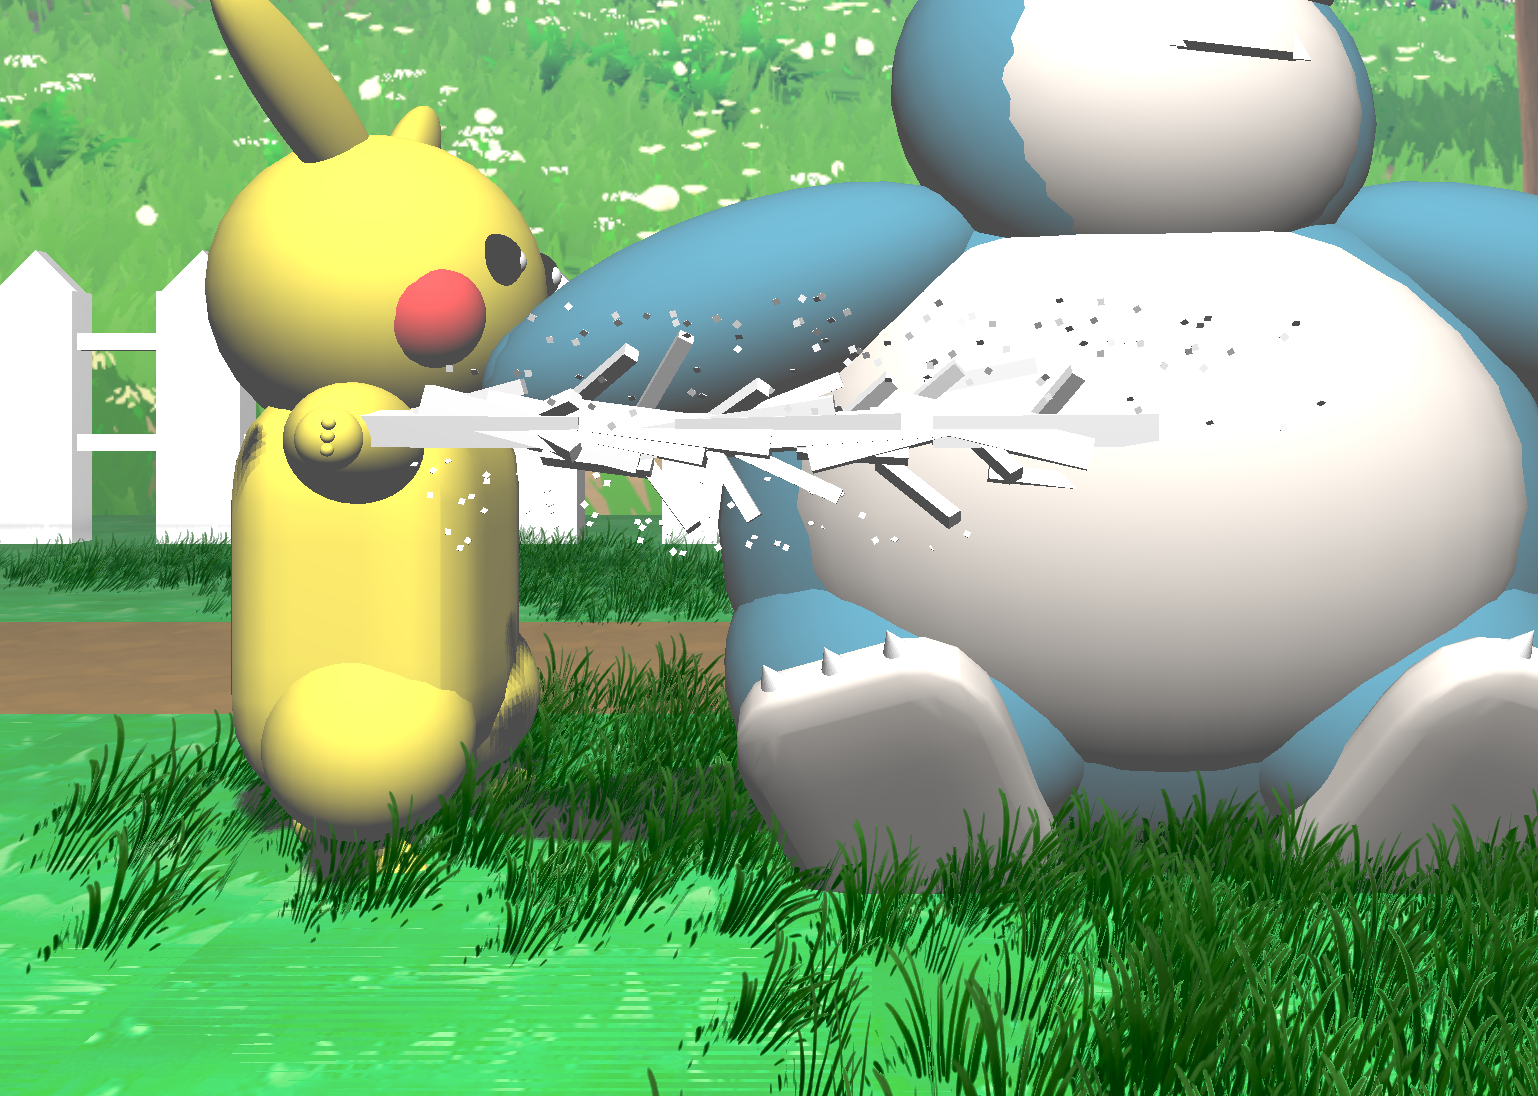
\includegraphics[width=100mm]{lightning.png} \\
    This beam is implemented mainly by 3 parts. The first part is the trunk of this beam, which consists of a random number of cubes with a random rotation from -30 to 30 degrees on 'x' axis;  
    the second part is the branches of the beam, which consists a random number of cubes with a random rotation from -90 to 90 degrees on 'x' axis;
    the third part is the electrons, which consists a random number of small squares with some random offset to the trunk.
    The beam will have a short lifetime (0.1s), such that the Discharge::update() will invoke this method at a high frequency to achieve realistic lightning effect.
    \item \textit{meteorite\_fall(base\_num)}: this is the routine that generates base\_num to 1.5 * base\_num of meteorites that will falling from the sky to the ground. \\
    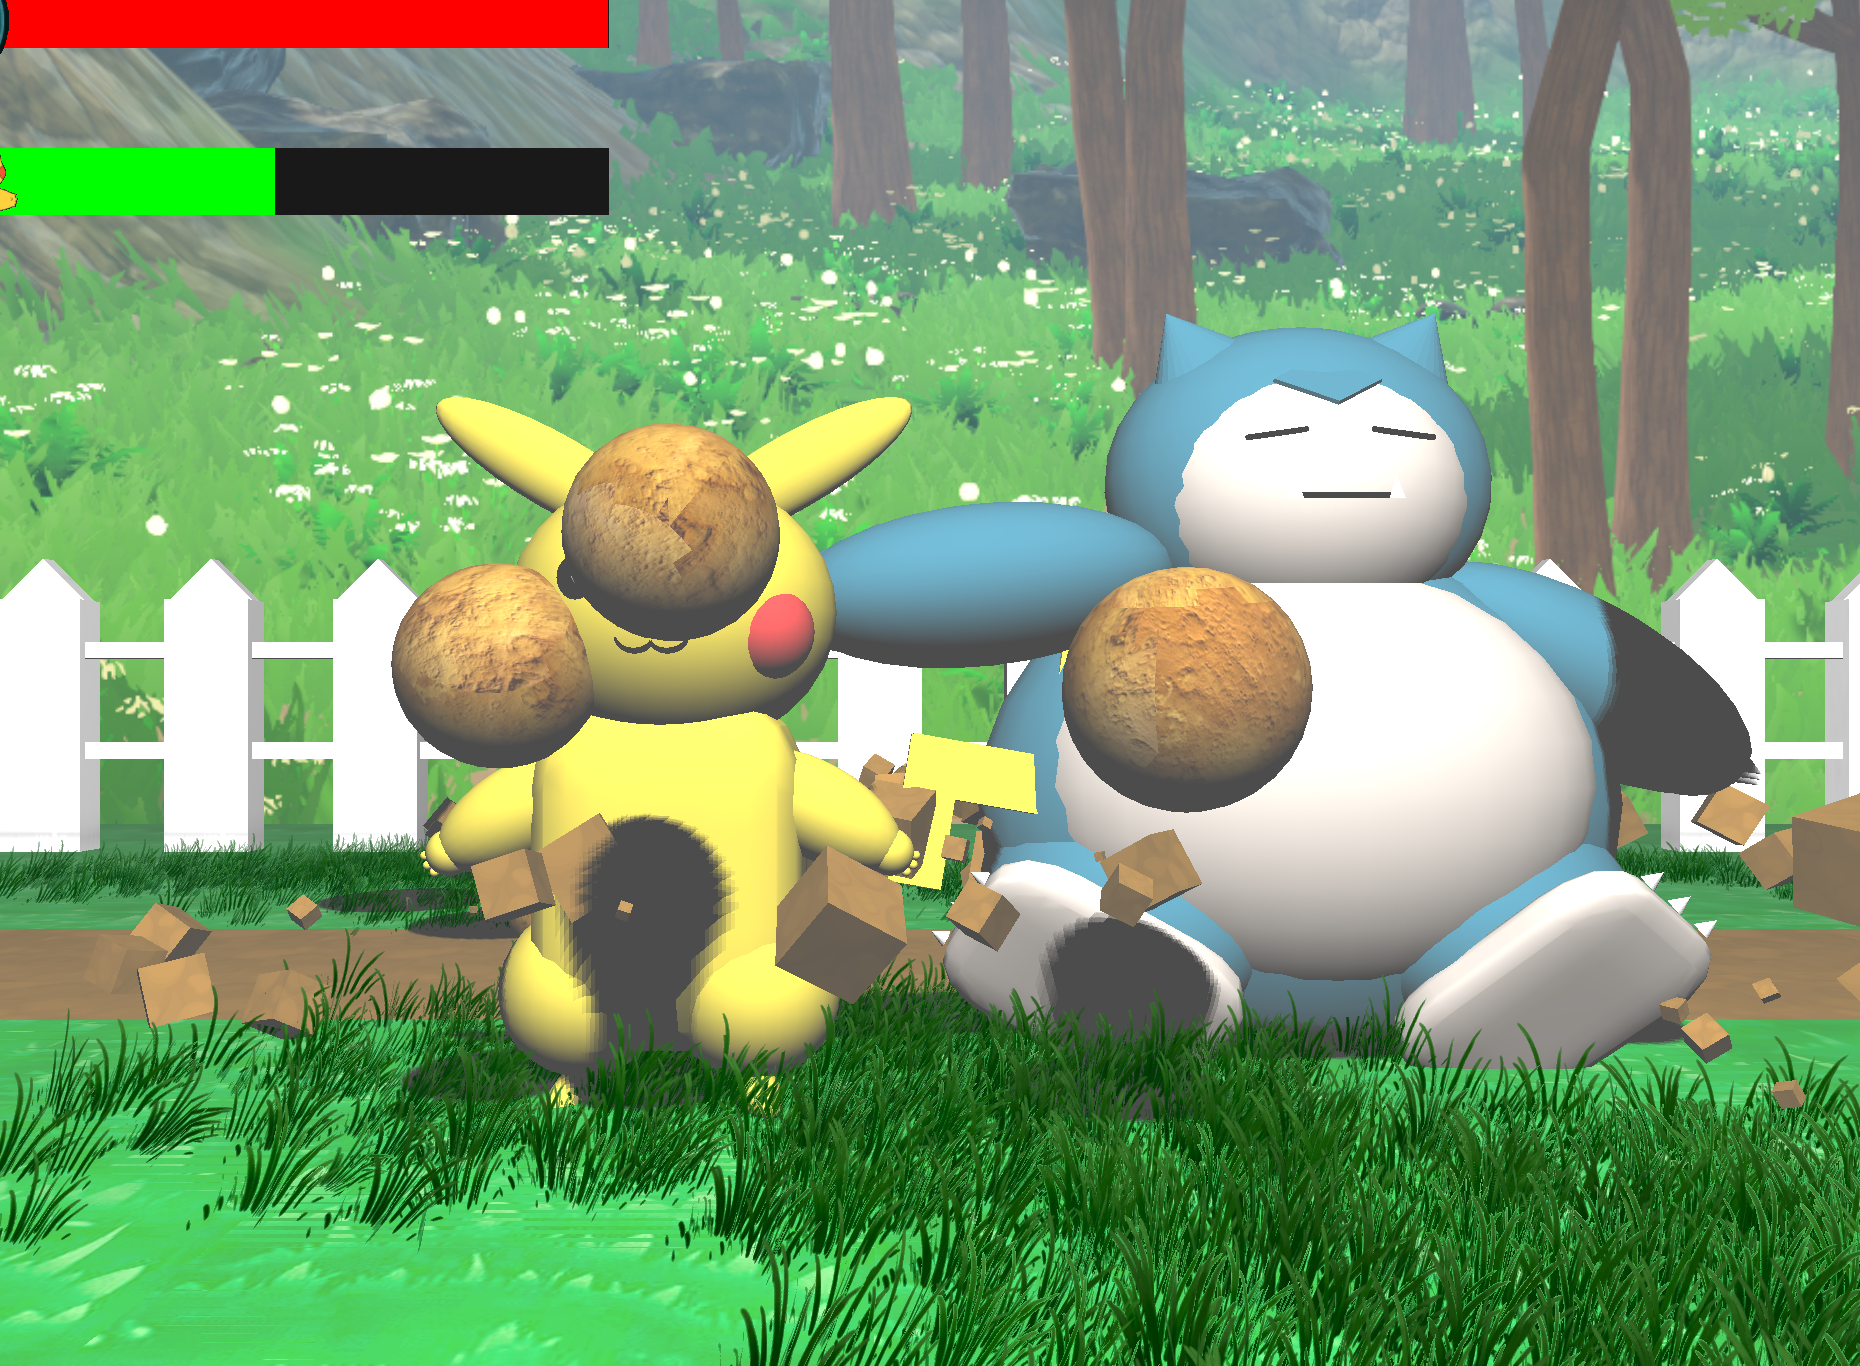
\includegraphics[width=100mm]{meteorite.png} \\ 
    This is implemented by randomly generate meteorite particles at x position from -50 to 50, y position from 30 to 150, z position from 0 to 100. Each meteorite will also be attached with a destroy function. When the meteorite is 
    destroyed (touched on the ground), the destroy function will be invoked and the following side effects will be performed: a flying dirt effect will be emitted at given position, if the meteorite hits Pikachu, the under\_attack method of Pikachu will be invoked
    to lower the hp. A camera shake will be performed.
    
\end{enumerate}
\subsection{Realistic Grass Rendering}
This section will discuss the implementation of realistic grass utilizing geometry shader. The high level idea of the implementation contains three parts
\begin{enumerate}
    \item We randomly generate points of the grass in the scene and pass to the vertex shader (grass.vs) using GL\_POINTS. Note that the vertex shader will not multiply the View and Perspective
    matrices to the points as usual, but it will directly pass the point to the geometry shader because the modelling of grass will be implemented at geometry shader's side(grass.geo).
    \item The geometry shader will take the point passed by the vertex shader and construct 3 crossed quad given that position. The cross effect is implemented by rotate a quad by 45 degrees of y axis.
    The creation of quad will also generate the uv coordinates of the each vertex of the quad that will be passed to the fragment shader for texture mapping.
    \item The wind effect is implemented by texture mapping of the flowmap. \\
    
\includegraphics[width=50mm]{flowmap.png} \\
    The red value of the image represents the direction in x, the green value of the image corresponds to the direction y, and the uv coordinates maps from the quad coordinates to the flowmap is calculated by the formula $uv = mod(\frac{base\_position.xz}{100.0} + windStrength * Time, 1.0)$, where the windStrength is 0.1f, Time is the 
    current time queried by \textit{glfwGetTime()}. This formula guarantees that grass at different position and at different timestamp will have different wind effects, which achieves the realism. \\
    Moreover, a 2D noise is added to the input of fragment shader to interpolate the color of grass from dark to light to achieve realism.
    \item The fragment shader will apply the texture  \\
    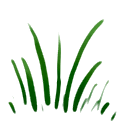
\includegraphics[width=50mm]{grass_texture.png} \\
    to each vertex emitted by the geometry shader. Note that there are some transparent part of this texture, so the fragment shader will discard the color if the 'a' component
    of the color after texture is less than 0.25. It will also interpolate the color between color and 0.5 * color by the noise factor passed by the geometry shader through the \textit{mix()} routine.
\end{enumerate}
This is the final effect of the grass: \\
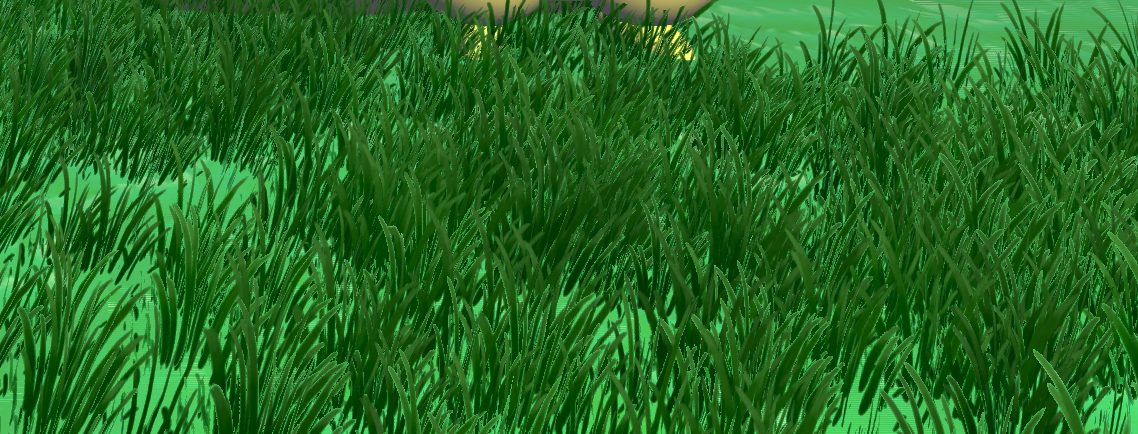
\includegraphics[width=100mm]{effect_grass.png}

\subsection{Additional features beyond the objective list}
To make this game complete, I also add some extra features:
\begin{enumerate}
    \item There is a start menu to let the user check the control manual, select the sound track and start the game. This is implemented by imgui
    \item There are hp bars for Pikachu and Snorlax indicating current hp of Pikachu and Snorlax. This is implemented by 3D rendering without Phong shading.
    When Pokemon are under attack, their related hp bar will be scaled and translated to achieve the effect of hp bar.
    \item Camera shakes are implemented to add the excitement of the game. This is completed by adding a noise to the original view and updates the view every frame.
    After the shake is over, the original view will be restored.
\end{enumerate}

\subsection{Lua Extension}
\begin{enumerate}
    \item \textbf{Texture:} to import a texture in Lua, you should write \textit{gr.texture("file.png")}, where file.png should be located in 
    "src/Assets/textures"; to apply a texture to a geometry node, you should write \textit{node.set\_texture(texture)}
    \item \textbf{Particle:} to add a particle system that emits particles using a geometry node, you should write \textit{node.set\_particle()}
    \item \textbf{Deep Copy:} to tile the scene with multiple geometry nodes, I developed a method named node.add\_child\_deepcpy(another) such that it will perform a deep copy on the other node 
    instead of directly points to it. This greatly boost my development of the scene because I can use a loop to add children into the scene.
\end{enumerate}

\newpage

\section{Others}
\subsection{Design Patterns \& Code}
\begin{enumerate}
    \item Singleton and Visitor design patterns are utilized in this project to improve the maintainability and extendability. 
    \item For objects that may traverse the SceneNode to perform some tasks, such as the GameWindow that will traverse the SceneNode to render the meshes,
    they only need to overwrite the visit(SceneNode*) method for a concrete SceneNode, then the recursive part happens automatically. 
    \item For objects that only appear once in this project and required to be accessed by multiple components, such as the Player class, Singleton pattern is utilized
    to lazily initialize the instance and offer interface for other components to access.   
    \item All the code are well commented and assertions are utilized completely to make sure the program executes correctly.
\end{enumerate}
\subsection{Debug Utilities}
in 'src/include/debug.hpp', I implemented some utilities for better debugging, if NDEBUG is defined by make config=release, 
DLOG and PRINT will have no effects; if NDEBUG is not defined (make config=debug), DLOG will perform the same to printf, while PRINT macro is for us to 
incorporate some debug statement, such as cout statement to print some objects like mat4 or vec3.\\
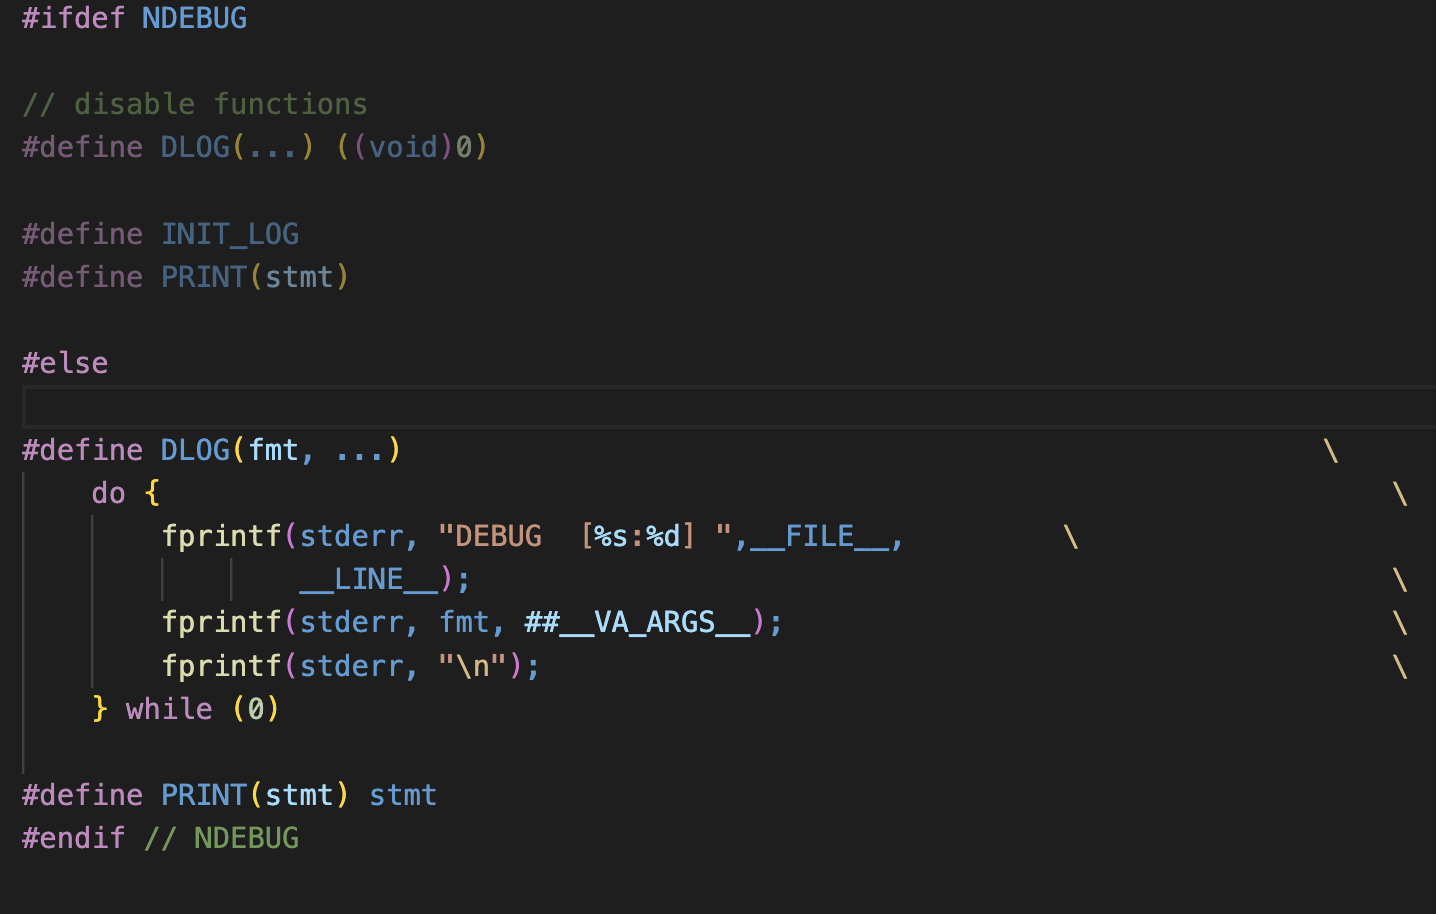
\includegraphics[width=100mm]{debug_code.png}
\subsection{Animation Assets Collection}
All animations are collected by the modified A3 program in /src/modelling, when we deselect a JointNode, its quaternion and translation will be printed out.


\newpage
\section{References}
\subsection{Assets References}
    All of the textures are free and retrieved from \url{https://www.textures.com/} \\
    All Pokemon background music are free and retrieved from the free video game music website \url{https://downloads.khinsider.com/game-soundtracks} \\
    Alll sound effects, including lightning and crushing, are purchased from the website \url{https://www.tukuppt.com/yinxiaomuban/dianji5781.html}
\subsection{Technical References}
\textit{Learn OpenGL - Graphics Programming}, de Vries, Joey, 2020. \\
    I use the web version at \url{https://learnopengl.com/} here are some specific articles:
    \begin{enumerate}
        \item \url{https://learnopengl.com/Guest-Articles/2020/Skeletal-Animation} for key-frame animation
        \item \url{https://learnopengl.com/Advanced-OpenGL/Cubemaps} for cube maps and texture mapping
        \item \url{https://learnopengl.com/In-Practice/2D-Game/Particles} for particle systems
        \item \url{https://learnopengl.com/Advanced-Lighting/Shadows/Shadow-Mapping} for shadow mapping
        \item \url{https://learnopengl.com/In-Practice/2D-Game/Audio} for 3D audio
    \end{enumerate}
    \textit{ GPU Gems: Programming Techniques, Tips, and Tricks for Real-Time Graphics}, Hubert Nguyen, 2007. \\
    I use the web version at \url{https://developer.nvidia.com/gpugems/gpugems/contributors}, and I learnt netural grass
    effect under the article \url{https://developer.nvidia.com/gpugems/gpugems/part-i-natural-effects/chapter-7-rendering-countless-blades-waving-grass}

\section{Acknowledgement}
    I would like to acknowledge that the 3D sound library utilizes the irrklang library, download at the official website \url{https://www.ambiera.com/irrklang/downloads.html} \\
    I would like to acknowledge that the 2D noise function used in src/Assets/grass.geo is based on \url{https://www.shadertoy.com/view/4dS3Wd} by morgan3d
\newpage



\noindent{\Large\bf Objectives:}

{\hfill{\bf Full UserID: z277zhu}\hfill{\bf Student ID:20817494}\hfill}

\begin{enumerate}
     \item[\_\_\_ 1:]  There is an environment mapping utilizing cubeMap to render a Pokemon skybox and a texture system to load and cache textures.

     \item[\_\_\_ 2:]  There is a 3D sound system that can both generate the background music and provide sound effect in the battle

     \item[\_\_\_ 3:]  There is a series of different animations utilizing transformation when the Pikachu and Snorlax are running, standing and attacking;  

     \item[\_\_\_ 4:]  There are particles simulating lightning and flying dirt when the two Pokemon attack

     \item[\_\_\_ 5:]  Toon shader is added, and there will be a button to switching from Toon shader or Phong shader.

     \item[\_\_\_ 6:]  Shadow mapping is added, and there will be a button to turn on/off the shadow mapping.

     \item[\_\_\_ 7:]  An artistic Pokemon scene will be rendered

     \item[\_\_\_ 8:]  realistic grass with wind effect is modeled by texture mapping and geometry shader

     \item[\_\_\_ 9:]  Snorlax AI is added

     \item[\_\_\_ 10:]  The Pikachu model in A3 will be upgraded and a Snorlax model will be created to support different motions.
\end{enumerate}

I would like to mention that for Objective 10, I planned to add a hip to Pikachu previously such that when the Pikachu is moving, he would transform from standing on two legs to standing on four legs, and
he would move forward with his four legs; however, when I implemented this, I found it extremely unnatural, so I removed the hip and add more details to the Pikachu's back.

% Delete % at start of next line if this is a ray tracing project
% A4 extra objective:
\end{document}